\chapter{Mass Moment of Inertia}

In this chapter the following assumptions are made
\begin{enumerate}
	\item Consider a body that rotates about the center of mass
	\item Use reference frames attached to the bodies
\end{enumerate}

Consider the following figure \ref{Fig_0_ch_5_MMI1}. The body frame and the reference frames are labeled as shown in figure \ref{Fig_0_ch_5_MMI1}. Consider a piece of mass $m_{i}$ which is at a distance $r_{i/A}$ from A. Angular momentum of this mass $m_{i}$ can be expressed as
\begin{equation}
	h_{i/A} = r_{i/A} \times p_{i/O}
\end{equation}
\begin{figure}[h!]
	\centering
	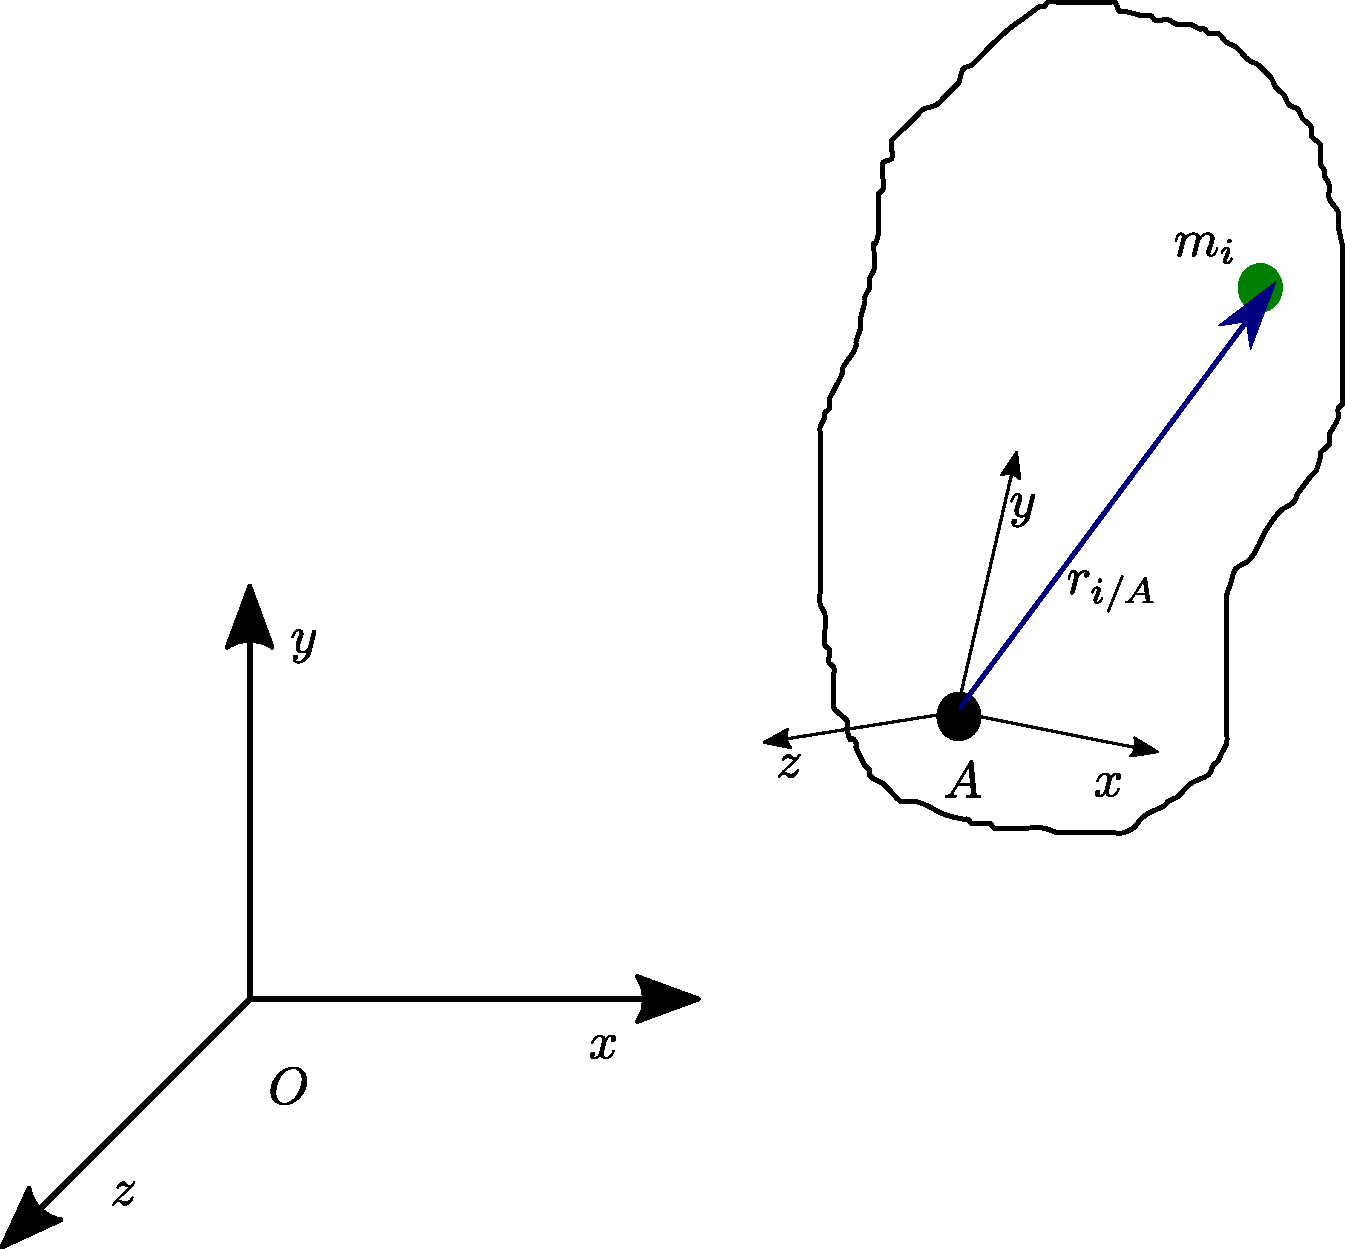
\includegraphics[width=0.6\linewidth]{Bilder/20_MMI_1.pdf}
	\caption{Finding mass moment of inertia (MMI)}
	\label{Fig_0_ch_5_MMI1}
\end{figure}

This problem is similar to the the one shown in figure \ref{Fig_0_ch_5_MMI2}. The problem can now be looked into using a specific know geometry. Since so far in this book, dynamics of only particles were discussed, this section servers as a starting point for the discussion on dynamics of rigid bodies. Here starting from simple known geometry to lay down foundational concepts, which can be extended later for specific applications of defining mass moment of inertia (MMI).
\newpage
\begin{figure}[h!]
	\centering
	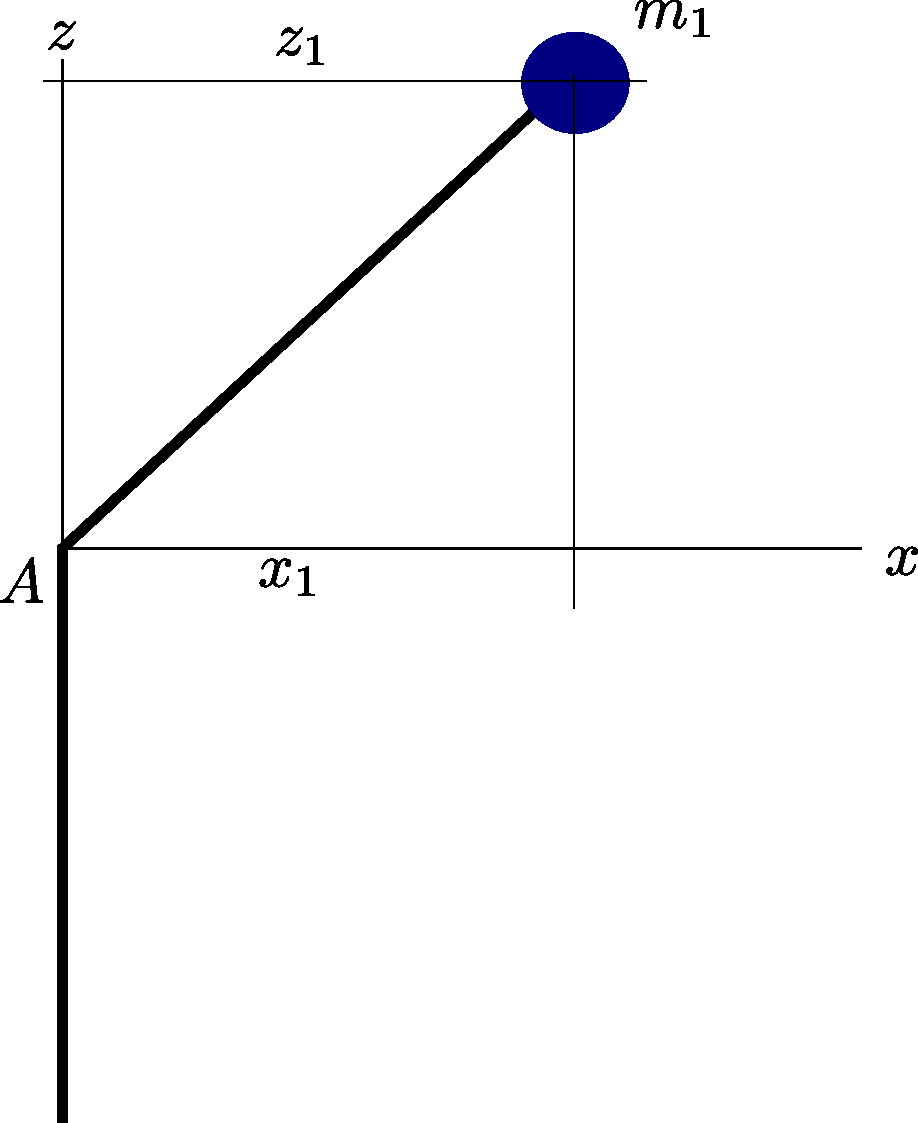
\includegraphics[width=0.6\linewidth]{Bilder/21_MMI_2.pdf}
	\caption{Similar problem on finding MMI}
	\label{Fig_0_ch_5_MMI2}
\end{figure}
using this geometry, the angular momentum of the mass $1$ attached can be found and grouped as follows:
\begin{align*}
	h_{1/A} &= r_{1/A} \times p_{1/O} = r_{1/A} \times m v_{1/O} \\
			&= \left( x_{1}\hat{i} + z_{1}\hat{k} \right) \times m_{1} {x}_{1}\omega \hat{j} \\
			&= m_{1}x_{1}^{2}\omega \hat{k} - m_{1}x_{1}z_{1}\hat{i}
\end{align*}
in the above equation, it can be see that the term $m_{1}x_{1}^{2}\omega \hat{k} = h_{z}$, angular momentum w.r.t $z$ axis, similarly, $m_{1}x_{1}z_{1}\hat{i} = h_{x}$. If the rigid body had a component along the $\hat{j}$ direction, then angular momentum $h_{y}$ would also be reflected in the above equation. Therefore, itseems that while find angular momentum and associated torques of a rigid body under circular motion is always accompanied by the components of angular momentum along all the three coordinate directions $x$, $y$ and $z$. Using this analogy, in general, it can be said that the angular momentum of a rigid busy is made up as follows
\begin{equation}\label{Eq_0_ch_5_angularmomentumRBs}
	H_{/A} = r_{/A} \times P_{/O}
\end{equation}
in equation \eqref{Eq_0_ch_5_angularmomentumRBs}, for rigid bodies, each term is now denoted using a capital letter (except for the radial vector). Also notice that for each of the term $H_{/A}$ or $P_{/O}$ the quantities are not referenced to any point, because for rigid bodies it is always reference to the center of mass, and the body as a whole.

\textbf{\textit{Note: }}It can be noted here that for all rigid body problems the velocity $v_{/O}$ always contains the part only due to $\omega \times r_{/O}$, as the distance between the particles in rigid bodies is always fixed, eliminating terms of relative velocities.

Equation \eqref{Eq_0_ch_5_angularmomentumRBs} can be proved by considering the rigid body as a system of particles with a center of mass $m_{T}$ and solving for the angular momentum equations from there
\begin{equation}
	H_{/A} = \sum_{i} r_{i/A} \times p_{i/O} = \sum_{i} m_{i} r_{i/A} \times \left( \omega \times r_{i/A} \right)
\end{equation}
which will result in
\begin{equation}
	H_{/A} = H_{x} \hat{i} + H_{y} \hat{y} + H_{z} \hat{k}
\end{equation}
where
\begin{align*}
	H_{x} &= I_{xx}\omega_{x} + I_{xy}\omega_{y} + I_{xz}\omega_{z} \\
	H_{y} &= I_{yx}\omega_{x} + I_{yy}\omega_{y} + I_{yz}\omega_{z} \\
	H_{z} &= I_{zx}\omega_{x} + I_{zy}\omega_{y} + I_{zz}\omega_{z} \\
\end{align*}
or can be written conveniently using matrix form:
\begin{equation} \label{Eq_0_ch_5_angularMomentum_matrixForm}
	\begin{bmatrix}
	H_{x} \\ H_{y} \\ H_{z}	\end{bmatrix} = \begin{bmatrix}
	I_{xx} \quad I_{xy} \quad I_{xz} \\
	I_{yx} \quad I_{yy} \quad I_{yz} \\
	I_{zx} \quad I_{zx} \quad I_{zz}
	\end{bmatrix} \begin{bmatrix}
			\omega_{x} \\ \omega_{y} \\ \omega_{z}
	\end{bmatrix}
\end{equation}

\section{Principal axes}

Every rigid body has axes through it such that the rotating about this axes does not produce any unbalanced torques on any other axes. However, care should be taken to note that the unbalanced torque does not in essence pertain to vibrations that result from center of mass being shifted from the axis os rotation. In this case of vibration, there is no unbalanced torque produced along any other axis of rotations, therefore, even though there is a vibration on the selected axis, it can be chosen as principal axis as it does not produce  any unbalanced torques on any other axes.

Consider equation \ref{Eq_0_ch_5_angularMomentum_matrixForm}, it can be seen that the only way to avoid producing any unbalanced torques on any other axes is making the off-diagonal elements to zero. Such that, angular momentum is only on one of these following axes $H_{x}$, $H_{y}$, $H_{z}$, when torque is applied on any of these axes. 

The key thing to remember about principal axes is that they should be chosen in a way so as to make the off-diagonal elements go to zero.

There are some simple ways to find principal axes using geometry
\begin{enumerate}
	\item If there is an axis of symmetry then that axis is a principal axis - circular objects have axis of symmetry about the center of circle. Axis of symmetry: An axis about which any point / object is equally reflected exactly across the axis as shown in figure \ref{Fig_0_ch_5_MMI3}
	\begin{figure}[h!]
		\centering
		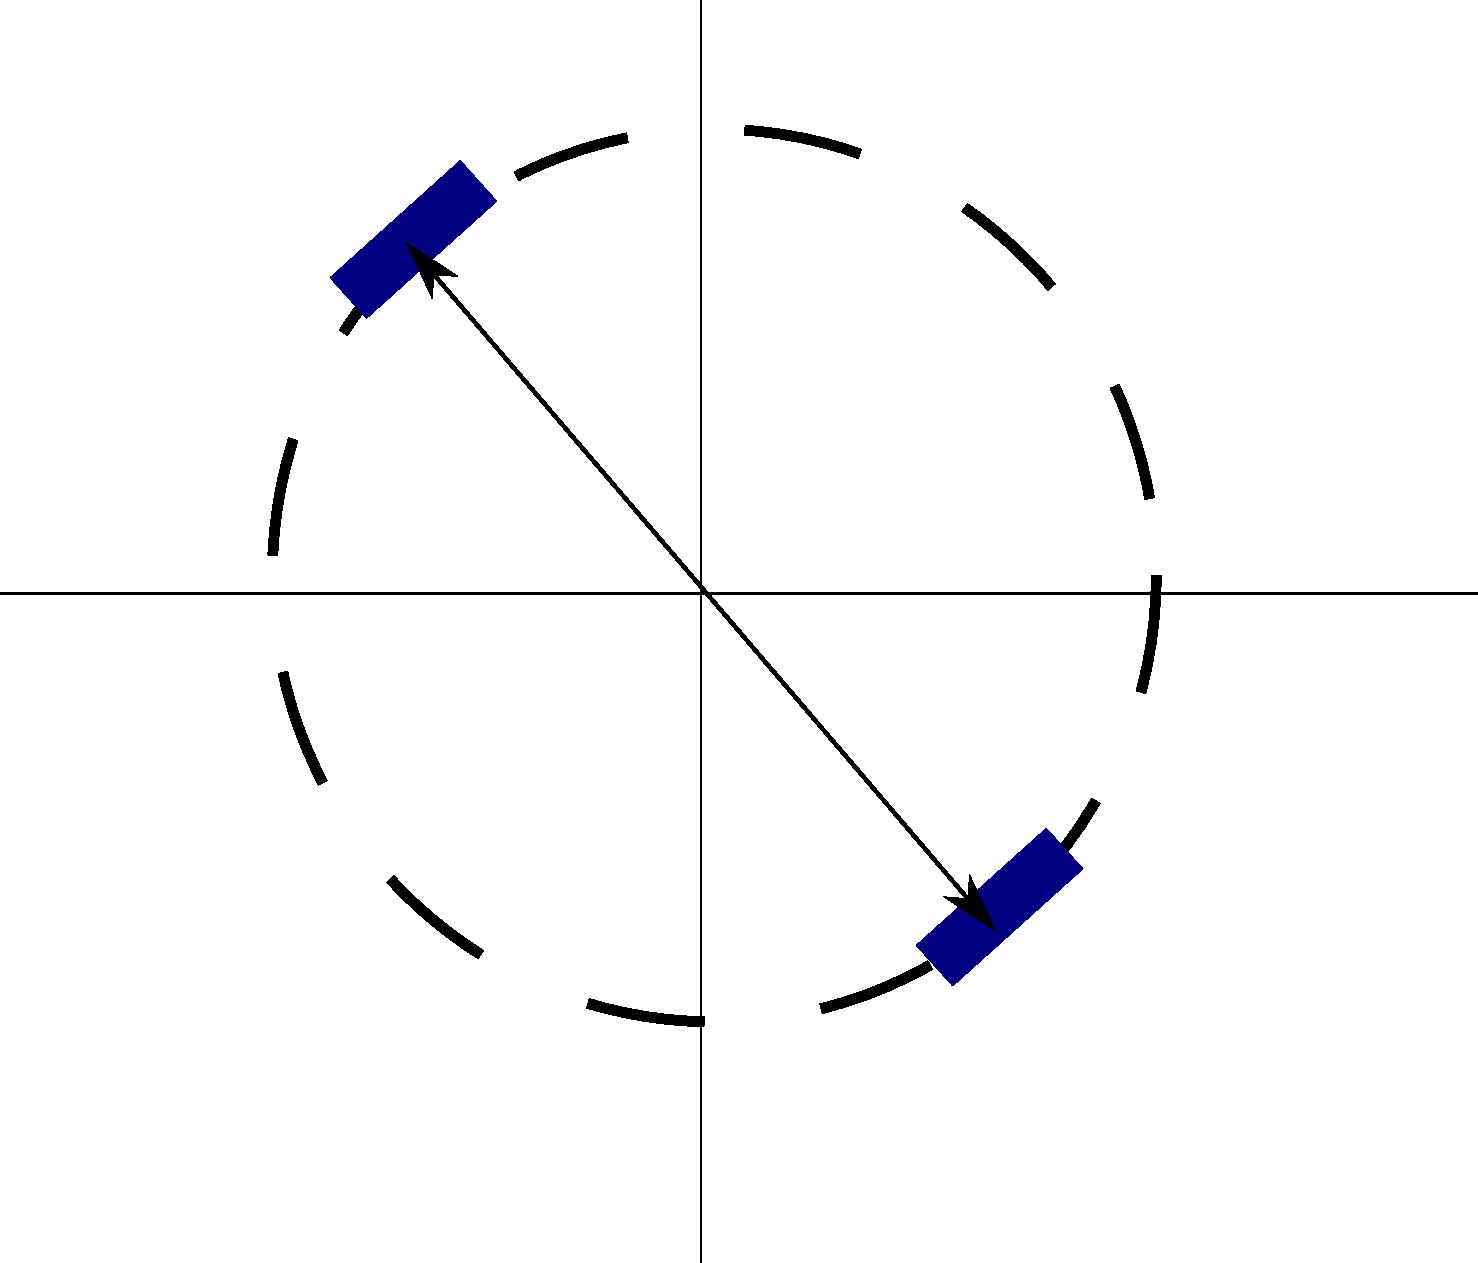
\includegraphics[width=0.4\linewidth]{Bilder/22_MMI3.pdf}
		\caption{Axis of symmetry for rotating objects}
		\label{Fig_0_ch_5_MMI3}
	\end{figure}

	\item If there is one plane of symmetry, then there is a principal axis perpendicular to it. Let it pass through center of mass $G$
	
	\item If there are two orthogonal planes of symmetry, their intersection is a principal axis. Principal axes are the property of an object.
\end{enumerate}

\section{Angular momentum of rigid bodies}

Extending the equations from the previous section, angular momentum for rigid bodies is expressed in matrix from by:
\begin{equation}
	H_{/A} = \left[I_{/A}\right]\begin{bmatrix}
		0 // 0 // \omega_{z}
	\end{bmatrix} = \begin{bmatrix}
		I_{xx} \quad I_{xy} \quad I_{xz} \\
		I_{yx} \quad I_{yy} \quad I_{yz} \\
		I_{zx} \quad I_{zx} \quad I_{zz}
	\end{bmatrix} \begin{bmatrix}
	\omega_{x} \\ \omega_{y} \\ \omega_{z}
	\end{bmatrix}
\end{equation}
In equation form, angular momentum for rigid bodies is expressed as:
\begin{equation}
	H_{/A} = H_{x} \hat{i} + H_{y} \hat{y} + H_{z} \hat{k}
\end{equation}
In the case when the I matrix has non-zero components along its off-diagonal elements, then angular momentum non-zero about the non-rotating axis, therefore, producing un-balanced torques along these non-rotating axes. This creates an imbalance of moments in the system. These off-diagonal elements are called products of inertia and are the cause for producing un-balanced torques about the non-rotating axis, as described in the following section \ref{Sec_ProdOfInertia}.

\textbf{\textit{Note: }} The one important factor for calculating $\vec{H}_{/A}$ for rigid bodies, is that here inertia matrix $\vec{I}$ for rigid bodies have to be considered.

\section{Products of inertia} \label{Sec_ProdOfInertia}

Consider figure \ref{fig_0_ch_5_prodOfInertia_1}, where the mass of an object is placed asymmetrically about the rotating axis.
\begin{figure}[h!]
	\centering
	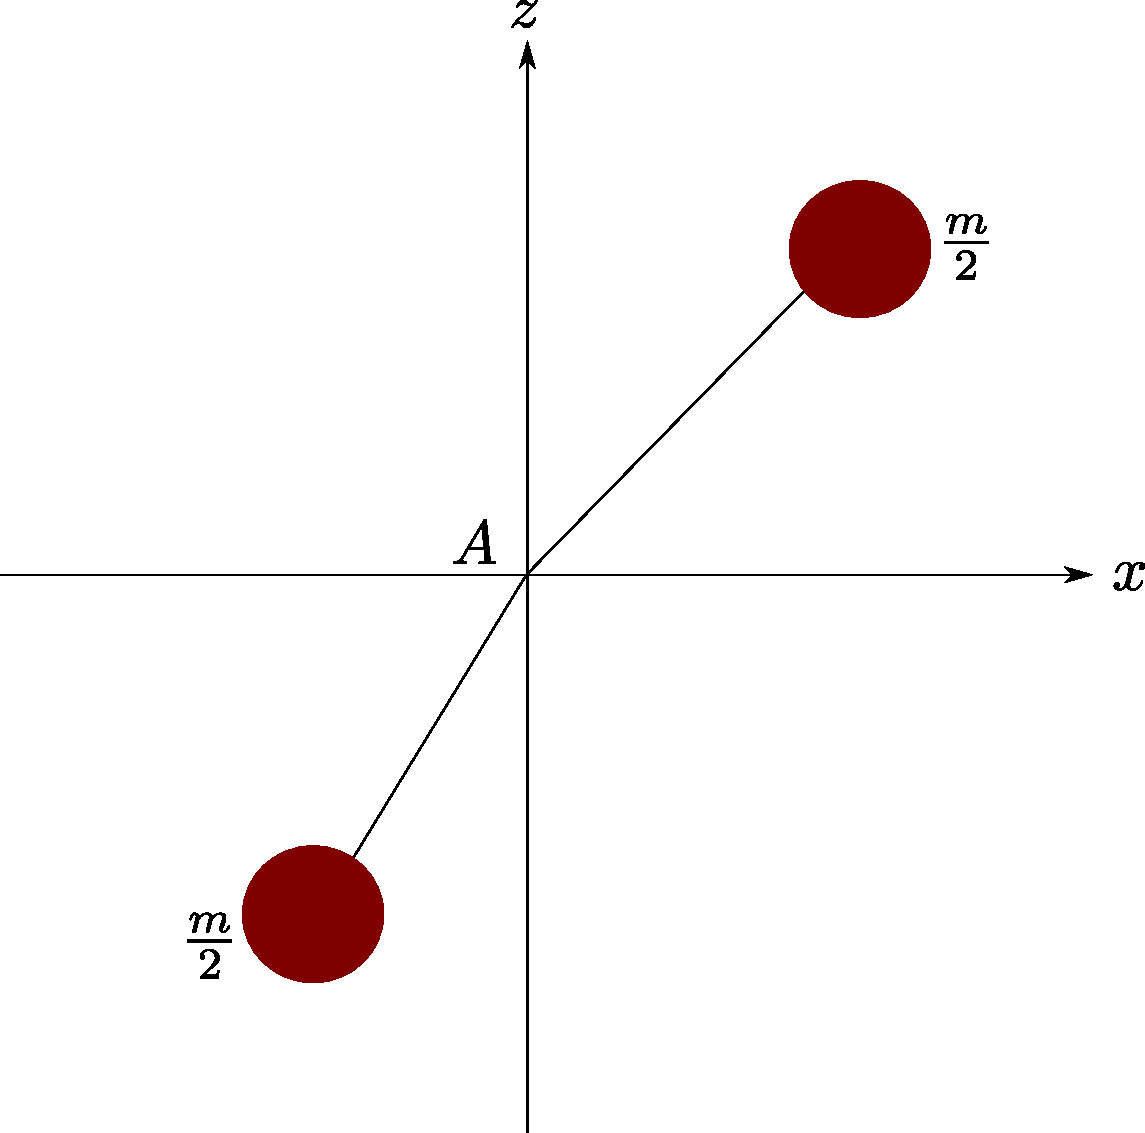
\includegraphics[width=0.5\linewidth]{Bilder/27_ProdOfInertia.pdf}
	\caption{Mass placed asymmetrically about the rotating axis}
	\label{fig_0_ch_5_prodOfInertia_1}
\end{figure}

I matrix can be computed using various standard methods described in dynamics texts, it will result in the following:
\begin{equation}
	\vec{I} = \begin{bmatrix}
		m z_{1}^{2} & 0 & -	m z_{1}z_{2} \\ 0 & m \left( x_{1}^{2} +  z_{1}^{2}\right) & 0 \\
		- m x_{1}z_{1} & 0 & m x_{1}^{2}
	\end{bmatrix}
\end{equation}

the rotation is only along $\omega_{z}$, therefore:
\begin{equation}
	\vec{H}_{/A} = \vec{I} \begin{bmatrix}
		0 \\ 0\\ \omega_{z}
	\end{bmatrix} = \begin{bmatrix}
		-m x_{1} z_{1}\omega_{z} \\ 0 \\ m x_{1}^{2} \omega_{z}
	\end{bmatrix} = \begin{bmatrix}
		H_{x} \\ H_{y} \\ H_{z}
	\end{bmatrix}
\end{equation}
torque about A van be expressed as:
\begin{equation}
	\vec{\tau}_{A} = \frac{d}{dt}\vec{H}_{/A} = \begin{bmatrix}
		-m x_{1} z_{1} \dot{\omega_{z}} \\ 0 \\ m x_{1}^{2} \dot{\omega_{z}}
	\end{bmatrix} = \begin{bmatrix}
		\tau_{x} \\ \tau_{y} \\ \tau_{z} 
	\end{bmatrix}
\end{equation}
It can be seen from the above expression, that due to off-diagonal elements in $\vec{I}$, there is a component of torque produced along the non-rotating $x$ axis. Therefore, products of inertia are the cause for producing un-balanced torques about the non-rotating axis.
\newpage
\begin{figure}[h!]
	\centering
	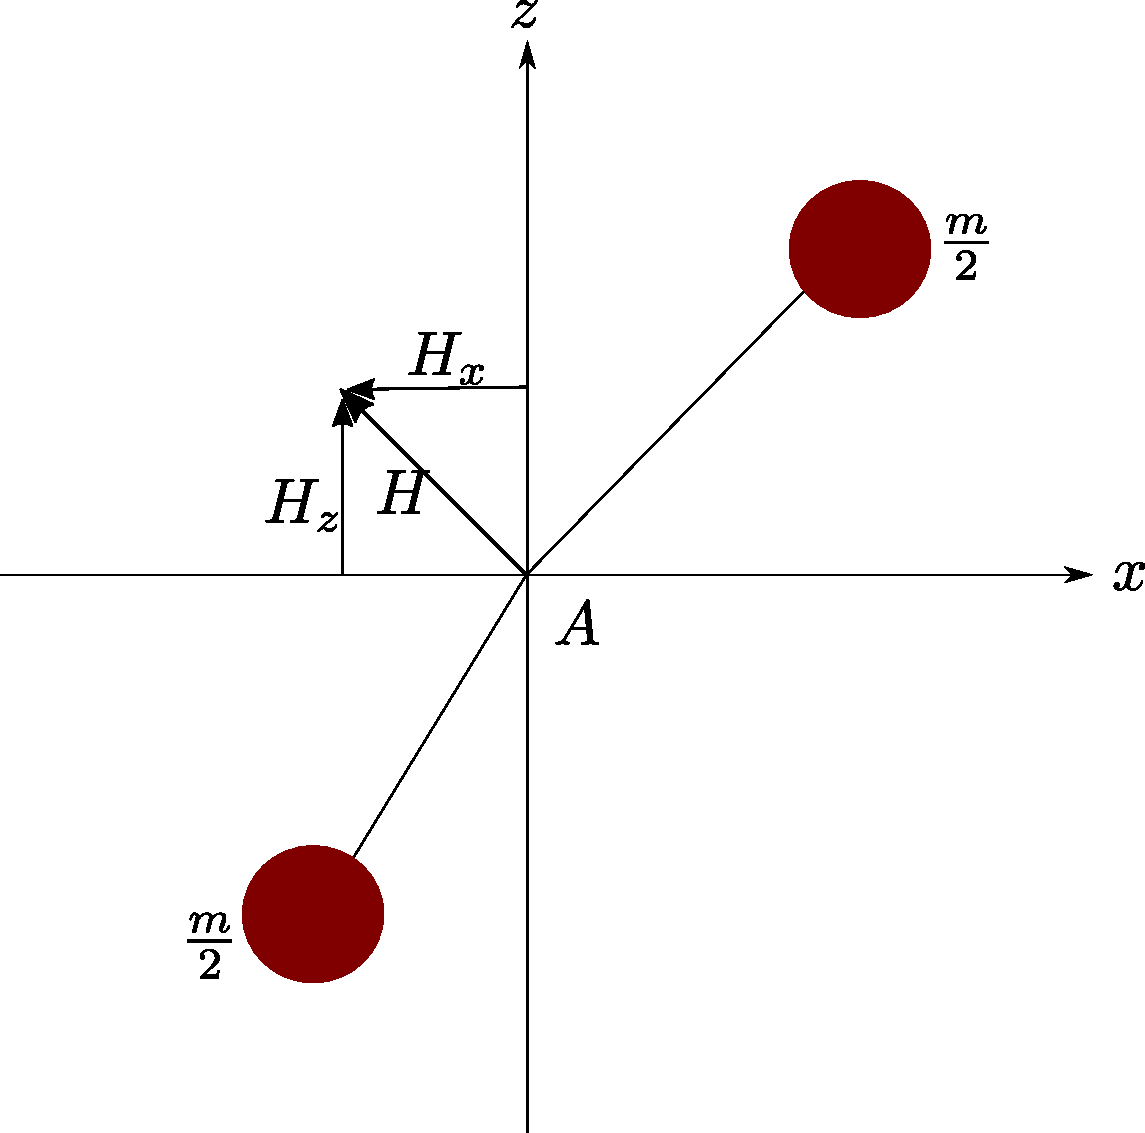
\includegraphics[width=0.5\linewidth]{Bilder/27_ProdOfInertia_1.pdf}
	\caption{Products of inertia results in $\vec{H}_{/A}$ on non-rotating axis}
	\label{fig_0_ch_5_H_NonRotatingAxis}
\end{figure}
Because $\vec{H}_{/A}$ is a vector, using vector addition, it can be shown using figure \ref{fig_0_ch_5_H_NonRotatingAxis}, how $\vec{H}_{/A}$ produces along the non-rotating axis. As $\vec{H}_{/A}$ is not pointing along the axis of rotation, therefore, it causes an imbalance.

\section{Exercise 1: Cart and pendulum problem}

Consider figure \ref{fig_0_ch_5_cadtAndPendulum1}
\begin{figure}[h!]
	\centering
	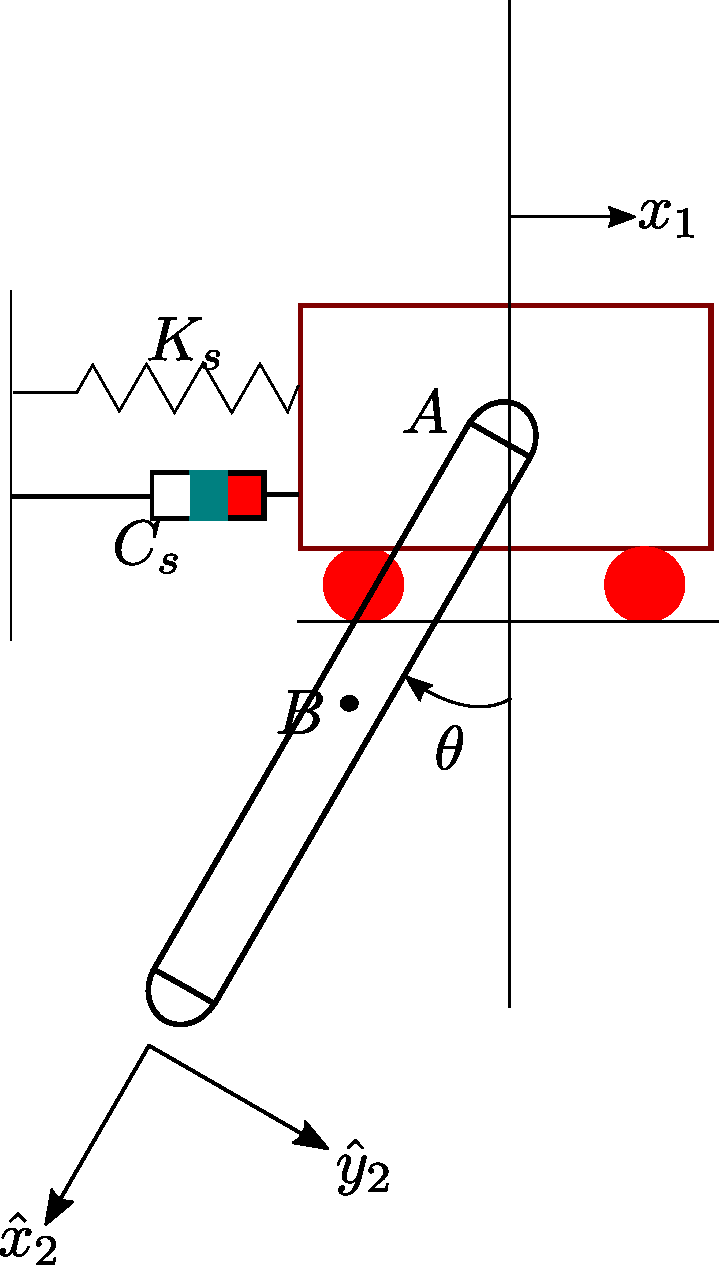
\includegraphics[width=0.5\linewidth]{Bilder/28_CartWithPendulum.pdf}
	\caption{Cart and pendulum}
	\label{fig_0_ch_5_cadtAndPendulum1}
\end{figure}

here, the problem is being solved considering that the pendulum is a rigid body with a diagonal $\vec{I}$ matrix, so that the angular momentum is calculated for a rigid body. 

\subsection{Coordinates}

Positive direction of cart is chosen as $x_{1}$, with coordinate $X_1 : \{ x_1, y_1, z_1 \}$. Pendulum angle is chosen $\theta$ about the vertical axis drawn straight from the point point A, and measured positive CCW. Further a coordinate $X_2 : \{ x_2, y_2, z_2 \}$ is chosen for the pendulum as shown in figure \ref{fig_0_ch_5_cadtAndPendulum1}. There are three possible distinct motions in this system, which have to be qualified using DOF and constraints.
\newpage
\subsection{DOF}

Listing the constraints:
\begin{enumerate}
	\item $y_1 = z_1 = 0$
	\item $M_{x1} = M_{y1} = M_{z1} = 0$
	\item $x_2 = z_2 = 0$
	\item $M_{x2} = M_{y2} = 0$
\end{enumerate}
there another holonomic constraint between $\theta$ and $\hat{y}_{2}$, such that $hat{y}_{2} = f(\theta)$, therefore, $C = 10$, $DOF = 12 - 10 = 2$. The possible coordinates are $\theta$ for the pendulums position and $x_1$ for the carts position. The EOMs should be formed as:
\begin{align}
	\sum F_{x1} &= m a_{A/0} \\
	\sum M_{/A} &= \frac{d}{dt}\vec{H}_{/A}  + v_{A/O} \times P_{B/O} \\
\end{align}

\subsection{External forces}

Using FBD for th pendulum, the following as shown in figure \ref{fig_0_ch_5_cadtAndPendulum2} can be produced. 
\begin{figure}[h!]
	\centering
	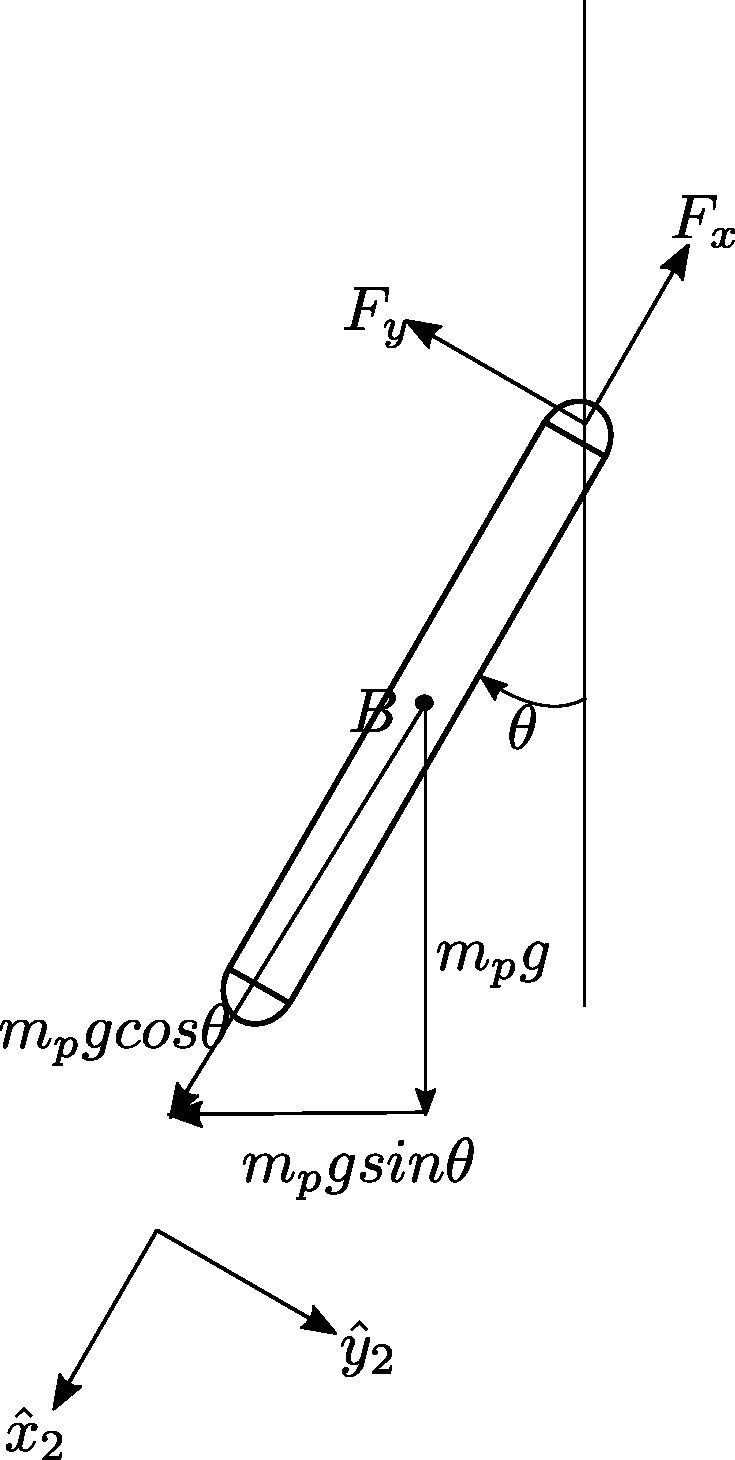
\includegraphics[width=0.35\linewidth]{Bilder/28_CartWithPendulum_FBD_Pend.pdf}
	\caption{FBD of pendulum}
	\label{fig_0_ch_5_cadtAndPendulum2}
\end{figure}
Apart from the components of $m_{p}g$ acting through $G$, reaction forces acting at A needs to be considered.
\textbf{\textit{Note: }}In figure \ref{fig_0_ch_5_cadtAndPendulum2}, the orientation of force $m_{p}gsin\theta$ is wrongly shown, it should be point in the direction parallel to $\hat{y}_{2}$. Also the direction of $\theta$ is shown wrong, in figure it is pointing to negative $\theta$.

Using figure \ref{fig_0_ch_5_cadtAndPendulum2}, moments about A can be expressed as (consider $l$ as the length of the pendulum):
\begin{equation}
	\sum M_{/A} = -m_{p} g \frac{l}{2} sin\theta \hat{k}_{1}
\end{equation}

finally, for forces along $\hat{x}_{1}$, consider the FBD for the cart as shown in figure \ref{fig_0_ch_5_cadtAndPendulum3}.
\begin{figure}[h!]
	\centering
	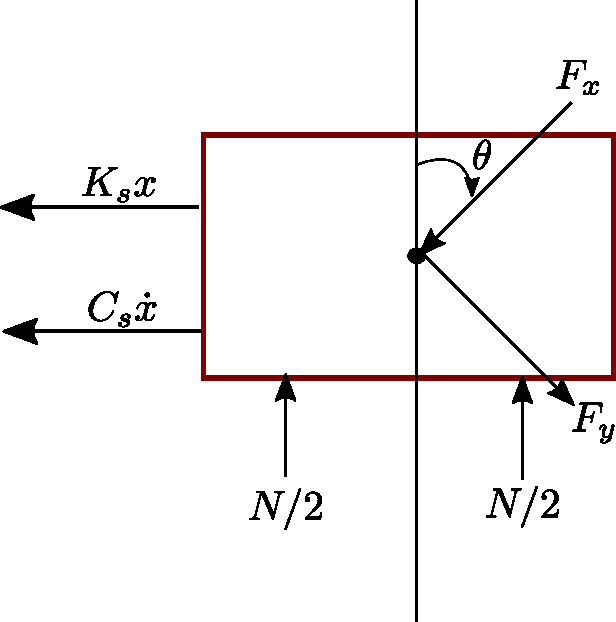
\includegraphics[width=0.35\linewidth]{Bilder/28_CartWithPendulum_FBD_Cart.pdf}
	\caption{FBD of cart}
	\label{fig_0_ch_5_cadtAndPendulum3}
\end{figure}
using figure \ref{fig_0_ch_5_cadtAndPendulum3}, balancing forces along $\hat{x}_{1}$ as:
\begin{equation} \label{eq_0ch_5_toBeAdded1}
	\sum F_{x1} = -K_{s}x - C_{s}\dot{x} - F_{x} sin\theta + F_{y} sin(\frac{\pi}{2} - \theta)
\end{equation}
where $\theta$ is the angle measure from the vertical line drawn straight from the pivot point A.

\textbf{\textit{Note: }}As the focus is only to find $\ddot{x}_{1}$, the forces that are acting only at the cart body need to be considered. Forces acting at the pendulum need not be considered, as by including reaction forces $F_{x}$ and $F_{y}$, the effect of pendulum has already been considered.

%In order to determine forces along $\hat{x}_{1}$ in cart and the pendulum, since there are forces acting in different body coordinates, it would be better at this point to use rotation matrices to simplify the task of finding the orientation of forces. In figure \ref{fig_0_ch_5_cadtAndPendulum2} and figure \ref{fig_0_ch_5_cadtAndPendulum3}, it can be seen that when $\theta = 0$, then the axes $\hat{x}_{1}$ and $\hat{x}_{2}$ are oriented by $\frac{3 \pi}{2}$ in positive $\theta$ this rotation will form the basis for DCM $\vec{R}_{1} = \vec{R(3\pi/2)}_{z}$, additionally, due to the rotation of the pendulum by $\theta$ there is another rotation matrix $\vec{R}(\theta)_{z}$.
%
%DCM $\vec{R}_{1}$ can be expressed as:
%\begin{equation}
%	\vec{R}_{1} = \vec{R(3\pi/2)}_{z} = \begin{bmatrix}
%		cos(3\pi/2) & sin(3\pi/2) & 0 \\ -sin(3\pi/2)  & cos(3\pi/2) & 0 \\ 0 & 0 & 1
%	\end{bmatrix}
%\end{equation}
%further, DCM $\vec{R}_{2}$ can be expressed as:
%\begin{equation}
%\vec{R}(\theta)_{z} = \begin{bmatrix}
%cos\theta & sin\theta  & 0 \\ -sin\theta  & cos\theta & 0 \\ 0 & 0 & 1
%\end{bmatrix}
%\end{equation}
%
%these two DCMs needs to be added in order to find the complete rotation of coordinate $X_{2}$ with reference to $X_{1}$,a composite rotation matrix property is user such that:
%\begin{align*}
%	\vec{R}_{2} &= [\vec{R}(\theta)_{z}][\vec{R}_{1}] \\
%				&= \begin{bmatrix}
%				cos\theta & sin\theta  & 0 \\ -sin\theta  & cos\theta & 0 \\ 0 & 0 & 1
%				\end{bmatrix}  \begin{bmatrix}
%				cos(3\pi/2) & sin(3\pi/2) & 0 \\ -sin(3\pi/2)  & cos(3\pi/2) & 0 \\ 0 & 0 & 1
%				\end{bmatrix} \\
%				&= \begin{bmatrix}
%				cos\theta cos(3\pi/2)- sin\theta sin(3\pi/2) & cos\theta sin(3\pi/2)+sin\theta cos(3\pi/2)  & 0 \\ -sin\theta cos(3\pi/2)-cos\theta sin(3\pi/2) & - sin\theta sin(3\pi/2) + cos\theta cos(3\pi/2) & 0 \\ 0 & 0 & 1
%				\end{bmatrix} \\
%	\begin{bmatrix} \hat{i}_{2} \\ \hat{j}_{2} \\ \hat{k}_{2} \end{bmatrix} &= \vec{R}_{2} \begin{bmatrix} \hat{i}_{1} \\ \hat{j}_{1} \\ \hat{k}_{1} \end{bmatrix} \\
%\end{align*}
%Using this above formulation, the two forces acting at the pendulums B $m_{p}g cos\theta$ and $m_{p}g sin\theta$ as well as two reaction forces $F_{x}$ and $F{y}$ which are all given in frame $X_{2}$ can be expressed in frame $X_{1}$, such that summation of forces can be calculated along the direction $\hat{x}_{1}$.
%
%Summation of forces (only pendulum) in coordinate $X_{2}$, expressed in frame $X_{1}$:
%\begin{equation}
%	\begin{bmatrix}
%	cos\theta cos(3\pi/2)- sin\theta sin(3\pi/2) & cos\theta sin(3\pi/2)+sin\theta cos(3\pi/2)  & 0 \\ -sin\theta cos(3\pi/2)-cos\theta sin(3\pi/2) & - sin\theta sin(3\pi/2) + cos\theta cos(3\pi/2) & 0 \\ 0 & 0 & 1
%	\end{bmatrix} \begin{bmatrix} m_{p}g cos\theta \\ -m_{p}g sin\theta \\ 0 \end{bmatrix}
%\end{equation}
%\begin{equation}
%	\begin{bmatrix}
%	cos\theta cos(3\pi/2)- sin\theta sin(3\pi/2)(+m_{p}g cos\theta)+cos\theta sin(3\pi/2)+sin\theta cos(3\pi/2)(-m_{p}g sin\theta) \\ -sin\theta cos(3\pi/2)-cos\theta sin(3\pi/2)(m_{p}g cos\theta) - sin\theta sin(3\pi/2) + cos\theta cos(3\pi/2)(-m_{p}g sin\theta) \\ 0
%	\end{bmatrix}
%\end{equation}
%Considering forces along $\hat{x}_{1}$:
%\begin{equation}\label{eq_0ch_5_toBeAdded2}
%	\sum F_{x1} = cos\theta cos(3\pi/2)- sin\theta sin(3\pi/2)(m_{p}g cos\theta)+cos\theta sin(3\pi/2)+sin\theta cos(3\pi/2)(-m_{p}g sin\theta)
%\end{equation}
%
%

\section{Finishing EOM}

we need to compute
\begin{equation}
\sum M_{/A} = \frac{d}{dt}\vec{H}_{/A}  + v_{A/O} \times P_{B/O}
\end{equation}
the left side of the equation is already been computed, the right side of the equation is computed as follows:
\begin{equation}
	v_{B/O} = v_{A/O} + v_{B/A} + \omega \times r_{B/A} = \dot{x}\hat{i}_{1} + 0 + \dot{\theta}\hat{k}_{1} \times \frac{l}{2}\hat{x}_{2}
\end{equation}
which is simplified to:
\begin{equation}
v_{B/O} = \dot{x}\hat{i}_{1} + \frac{l}{2}\dot{\theta} \hat{j}_{2}
\end{equation}
the linear momentum can therefore be calculated as:
\begin{equation}
	P_{B/O} = m \left( \dot{x}\hat{i}_{1} + \frac{l}{2}\dot{\theta} \hat{j}_{2} \right)
\end{equation}
the angular momentum about A can be expressed as:
\begin{equation}
	H_{/A} = \vec{I}_{A} \begin{bmatrix}
		0 \\ 0 \\ \omega_{z}\hat{k}_{1}
	\end{bmatrix} = \begin{bmatrix}
	0 & 0 & 0 \\ 0 & 0 & 0 \\ 0 & 0 & \frac{1}{3}m l^{2}
	\end{bmatrix}\begin{bmatrix}
	0 \\ 0 \\ \omega_{z}\hat{k}_{1}
	\end{bmatrix} = \frac{1}{3}m l ^{2} \dot{\theta} \hat{k}_{1}
\end{equation}
finally, computing $\frac{d}{dt}\vec{H}_{/A}  + v_{A/O} \times P_{B/O}$:
\begin{equation}
	\frac{d}{dt}\vec{H}_{/A}  + v_{A/O} \times P_{B/O} = \frac{1}{3}m l ^{2} \ddot{\theta} \hat{k}_{1} + \dot{x}_{1}\hat{i}_{1} \times m \left( \dot{x}_{1}\hat{i}_{1} + \frac{l}{2}\dot{\theta} \hat{j}_{2} \right)
\end{equation}
there needs to be a relationship established between $\hat{i}_{1}$ and $\hat{j}_{2}$, by working out the orientations of the unit vectors, it can be found that:
\begin{align*}
	\hat{i}_{2} &= sin\theta \hat{i}_{1} + cos \theta \hat{j}_{1} \\
	\hat{j}_{2} &= -sin \theta \hat{j}_{1} + cos \theta \hat{i}_{1}
\end{align*}
using this in the above expression and simplifying the result, leads to,
\begin{equation}
\frac{d}{dt}\vec{H}_{/A}  + v_{A/O} \times P_{B/O} = \frac{1}{3}m l ^{2} \ddot{\theta} \hat{k}_{1} - m sin\theta \dot{x}_{1} \dot{\theta} \frac{l}{2} \hat{k}_{1} 
\end{equation}
Equating both sides of the EOM,
\begin{equation*}
	- m_{p} g \frac{l}{2} sin\theta \hat{k}_{1} = \frac{1}{3}m l ^{2} \ddot{\theta} \hat{k}_{1} - m sin\theta \dot{x}_{1} \dot{\theta} \frac{l}{2} \hat{k}_{1}
\end{equation*}
solving the equation for $\ddot{\theta}$:
\begin{equation} \label{eq_0_ch_5_EOM1}
	\ddot{\theta} = \frac{m_{p} sin\theta \dot{x}_{1} \dot{\theta} \frac{l}{2} - m_{p} g \frac{l}{2} sin\theta}{\frac{1}{3}m_{p} l ^{2}} = \frac{\left(sin\theta \frac{l}{2}\right)  \left(\dot{x}_{1} \dot{\theta} - g\right) }{\frac{1}{3} l ^{2}}
\end{equation}

EOM for $\ddot{x}_{1}$ is expressed as (using equation \eqref{eq_0ch_5_toBeAdded1}):
\begin{equation}
	-K_{s}x - C_{s}\dot{x} - F_{x} sin\theta + F_{y} sin(\frac{\pi}{2} - \theta) = m \ddot{x}_{1}
\end{equation}
solving the above equation for $\ddot{x}_{1}$:
\begin{equation}\label{eq_0_ch_5_EOM2}
	\ddot{x}_{1} = \frac{1}{m_{c}} \left[	-K_{s}x - C_{s}\dot{x} - F_{x} sin\theta + F_{y} sin(\frac{\pi}{2} - \theta)\right]
\end{equation}
where $m_{c}$ is the mass of the cart and $m_{p}$ is the mass of the pendulum. Equations \eqref{eq_0_ch_5_EOM1} and \eqref{eq_0_ch_5_EOM2} form the EOMs for this pendulum-cart system.

In equation \eqref{eq_0_ch_5_EOM2}, there are reaction forces $F_{x}$ and $F_{y}$, that needs to be determined, in order for the system description to be complete. Since $F_{x}$ and $F_{y}$ are the reaction forces generated due to pendulums motion, $F_{x}$ and $F_{y}$ can be found using figure \ref{fig_0_ch_5_cadtAndPendulum2}. 

Equating forces along $\hat{x_{2}}$,
\begin{equation}\label{eq_0_ch_5_random22}
	\sum F_{x2} = -F_{x} + m_{p} g cos\theta = m a_{B/O} \hat{x_{2}}
\end{equation}
$a_{B/O}$ from the expression above needs to be calculated,
\begin{equation}
	a_{B/O} = a_{A/O} + \prescript{A}{}{a_{B/A}} + \left[2\omega_{/O} \times v_{B/A}\right] + \left[\dot{\omega}_{/O} \times r_{B/A}\right] + \left[\omega_{/O} \times \left(\omega_{/O} \times r_{B/A}\right)\right]
\end{equation}
from the expression of $a_{B/O}$, the terms $\prescript{A}{}{a_{B/A}} = 0$ as B is fixed relative to A. Therefore, reducing the expressed for $a_{B/O}$ to as follows
\begin{equation}
a_{B/O} = a_{A/O} + \left[2\omega_{/O} \times v_{B/A}\right] + \left[\dot{\omega}_{/O} \times r_{B/A}\right] + \left[\omega_{/O} \times \left(\omega_{/O} \times r_{B/A}\right)\right]
\end{equation}
additionally, the term $v_{B/A}$ needs to be found,
\begin{equation}
	v_{B/A} = \prescript{A}{}{v_{B/A}} + \omega_{/O} \times r_{B/A} = 0 + \dot{\theta}\hat{k}_{1} \times \frac{l}{2}\hat{x}_{2} = \frac{l}{2}\dot{\theta}\hat{j}_{2}
\end{equation}
substituting $v_{B/A}$ in expression for $a_{B/A}$,
\begin{equation}\label{eq_0_ch_5_random21}
a_{B/O} = \ddot{x}_{1}\hat{x}_{1} + \left[2\dot{\theta}\hat{k}_{1} \times \frac{l}{2}\dot{\theta}\hat{y}_{2}\right] + \left[\dot{\theta}\hat{k}_{1} \times \frac{l}{2}\hat{x}_{2}\right] + \left[\dot{\theta}\hat{k}_{1} \times \left(\dot{\theta}\hat{k}_{1} \times \frac{l}{2}\hat{x}_{2}\right)\right]
\end{equation}
simplifying the above terms,
\begin{itemize}
	\item $\left[2\dot{\theta}\hat{k}_{1} \times \frac{l}{2}\dot{\theta}\hat{y}_{2}\right] = - l \dot{\theta}^{2} \hat{y}_{2}$
	\item $\left[\ddot{\theta}\hat{k}_{1} \times \frac{l}{2}\hat{x}_{2}\right] = \frac{l}{2}\ddot{\theta}\hat{y}_{2}$
	\item $\left[\dot{\theta}\hat{k}_{1} \times \left(\dot{\theta}\hat{k}_{1} \times \frac{l}{2}\hat{x}_{2}\right)\right] = - \frac{l}{2}\dot{\theta}^{2} \hat{x}_{2}$
\end{itemize}
Note that in equation \eqref{eq_0_ch_5_random21}, there is a term with $\hat{x}_{1}$, which needs to be translated to $\hat{x}_{2}$ and $\hat{y}_{2}$. Performing the unit vector orientations carefully, it can be seen that the following relationship is true:
\begin{align}
	\hat{x}_{2} &= sin\theta \hat{x}_{1} + cos\theta \hat{y}_{1} \\
	\hat{y}_{2} &= -sin\theta \hat{y}_{1} + cos\theta \hat{x}_{1} \\
\end{align}
the above relationship can be expressed in form of rotation matrix as follows:
\begin{equation}
	\begin{bmatrix}
	\hat{x}_{2} \\ \hat{y}_{2} \\ \hat{z}_{2}
	\end{bmatrix} = \begin{bmatrix}
				sin\theta_{s} & cos\theta_{s} & 0 \\
				cos\theta_{s} & -sin\theta_{s} & 0 \\
				0 & 0 & 1
	\end{bmatrix}\begin{bmatrix}
	\hat{x}_{1} \\ \hat{y}_{1} \\ \hat{z}_{1}
	\end{bmatrix} = \prescript{X2}{X1}{\vec{R}} \begin{bmatrix}
	\hat{x}_{1} \\ \hat{y}_{1} \\ \hat{z}_{1}
	\end{bmatrix}
\end{equation}
where in $\prescript{X2}{X1}{\vec{R}}$, subscript $X1$ represents the base frame and $X2$ represents the follower frame. $\theta_{s}$ represents the angle measure from the vertical to $F_{x}$ as shown in figure \ref{fig_0_ch_5_cadtAndPendulum3}. Therefore, $\prescript{X2}{X1}{\vec{R}} = ^{T}\left[\prescript{X1}{X2}{\vec{R}}\right]$, which is expressed as,
\begin{equation}
	\begin{bmatrix}
	\hat{x}_{1} \\ \hat{y}_{1} \\ \hat{z}_{1}
	\end{bmatrix} = \begin{bmatrix}
		sin\theta_{s} & cos\theta_{s} & 0 \\
		cos\theta_{s} & -sin\theta_{s} & 0 \\
		0 & 0 & 1
	\end{bmatrix}\begin{bmatrix}
	\hat{x}_{2} \\ \hat{y}_{2} \\ \hat{z}_{2}
	\end{bmatrix}
\end{equation}
therefore, the term $\ddot{x}_{1}\hat{x}_{1} = \ddot{x}_{1} sin\theta_{s} \hat{x}_{2} + \ddot{x}_{1} cos\theta_{s} \hat{y}_{2} $, substituting this in equation \eqref{eq_0_ch_5_random21},
\begin{equation}\label{eq_0_ch_5_random23}
	a_{B/O} = \ddot{x}_{1} sin\theta_{s} \hat{x}_{2} + \ddot{x}_{1} cos\theta_{s} \hat{y}_{2} - l \dot{\theta}^{2} \hat{y}_{2} + \frac{l}{2}\ddot{\theta}\hat{y}_{2} - \frac{l}{2}\dot{\theta}^{2} \hat{x}_{2}
\end{equation}
equating equation \eqref{eq_0_ch_5_random23} with equation \eqref{eq_0_ch_5_random23}, the reaction forces can be found
\begin{equation*}
	-F_{x} + m_{p} g cos\theta = m_{p} \left(\ddot{x}_{1} sin\theta_{s}- \frac{l}{2}\dot{\theta}^{2}\right)
\end{equation*}
solving for $F_{x}$,
\begin{equation}
F_{x} = m_{p} \left(\frac{l}{2}\dot{\theta}^{2} + g cos\theta - \ddot{x}_{1} sin\theta_{s} \right)
\end{equation}


\section{Exercise 2: Translating System}

Consider a translating system as shown in figure \ref{fig_0_ch_5_translatingMasses1}. 
\begin{figure}[h!]
	\centering
	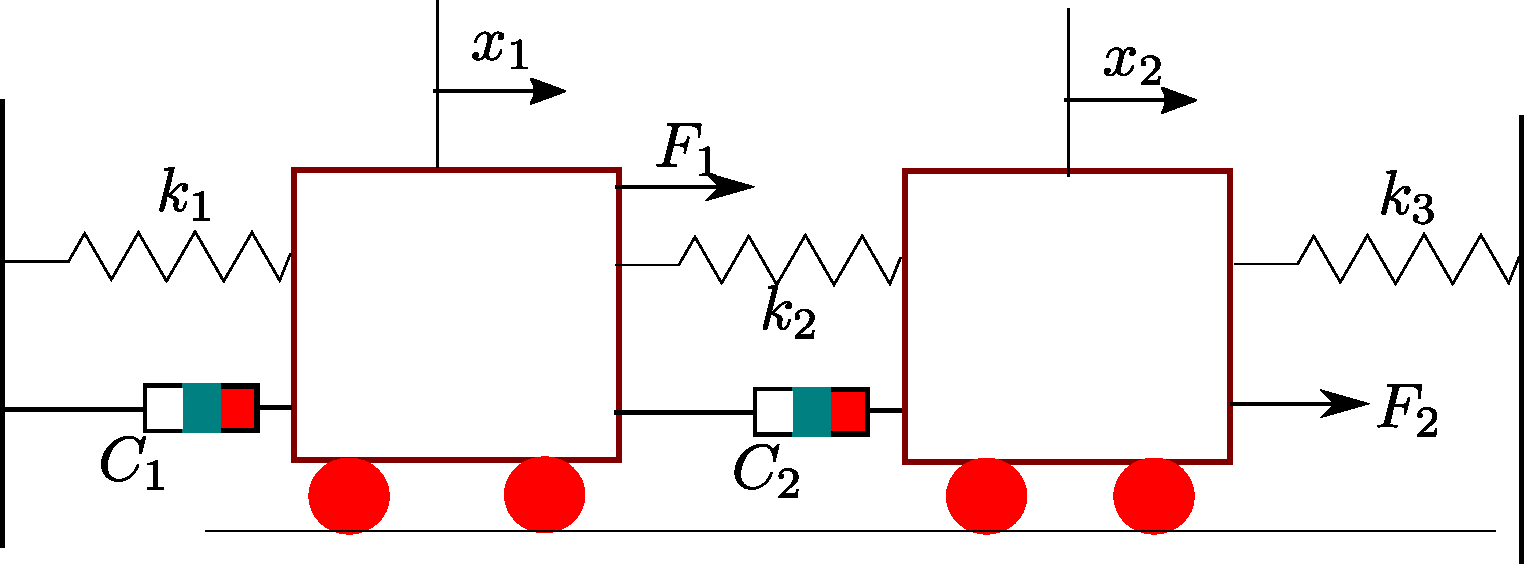
\includegraphics[width=0.5\linewidth]{Bilder/29_translatingMasses.pdf}
	\caption{Translating masses}
	\label{fig_0_ch_5_translatingMasses1}
\end{figure}

\subsection{Coordinate selection}
Choosing coordinates are quite straight forward in this problem. As shown in figure \ref{fig_0_ch_5_translatingMasses1}, both the masses $m_1$ and $m_2$ are allowed to translate only along $x_1$ and $x_2$ directions.

\subsection{DOF}
Since there are only two independent coordinate motions possible, there should be $C = 2\cdot6 - 2 = 10$ constraint placed in the system. This can be explained as follows
\begin{itemize}
	\item $y_1 = y_2 = z_1 = z_2 = 0$
	\item $M_{x1} = M_{x2} = M_{y1} = M_{y2} = M_{z1} = M_{z2} = 0$
\end{itemize}
Therefore, the EOMs should be of the form
\begin{align}
	\sum F_{x1} &= m a_{x1/O}\\
	\sum F_{x2} &= m a_{x2/O}\\
\end{align}

\subsection{External forces}

In order to determine the external forces on the system, each of the individual masses needs to be considered. Consider figure \ref{fig_0_ch_5_translatingMasses2}.
\begin{figure}[h!]
	\centering
	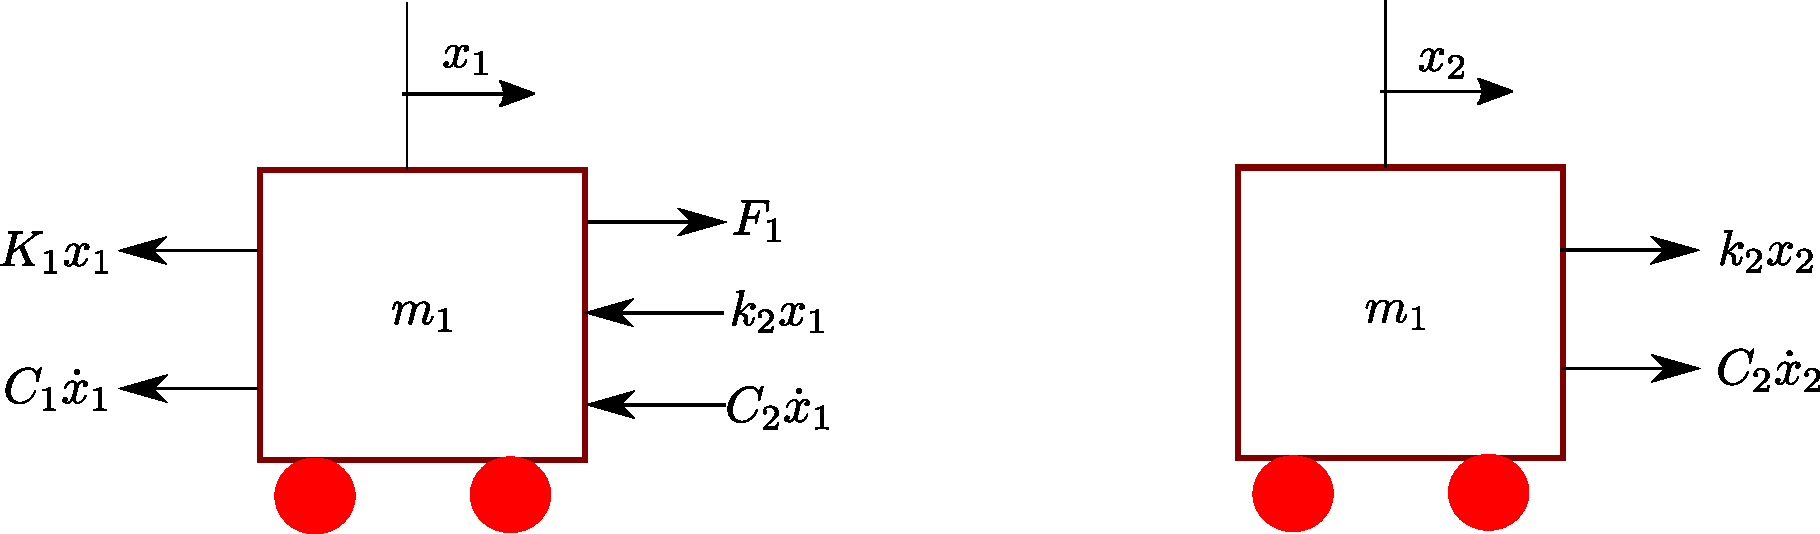
\includegraphics[width=0.5\linewidth]{Bilder/29_translatingMasses_FBD.pdf}
	\caption{FBD of mass 1}
	\label{fig_0_ch_5_translatingMasses2}
\end{figure}


